\section{FSA-v5 Model Specification and Identifiability Analysis} \label{sec:fsa-v5-fim}

This section is the canonical, self-contained specification of the FSA-v5 model in its current form, immediately followed by a Fisher-information identifiability analysis. The motivation is concrete: the model has evolved substantially since the v2-era identifiability work, and before importing the codebase into the \texttt{smc2fc} repository we need to know which parameters are well-constrained by the available observation channels and which are structurally over-parameterised or weakly informed.

\subsection{Full FSA-v5 equations in one place} \label{sec:v5-equations}

\paragraph{Latent state (6D).} $y(t) = (B, S, F, A, K_{FB}, K_{FS})^T$ with
\begin{itemize}
  \item $B \in [0,1]$ — aerobic fitness (Banister chronic; Jacobi diffusion).
  \item $S \in [0,1]$ — strength capacity (Banister chronic; Jacobi diffusion).
  \item $F \in [0, \infty)$ — unified fatigue pool (CIR diffusion).
  \item $A \in [0, \infty)$ — autonomic amplitude (Stuart--Landau; CIR diffusion).
  \item $K_{FB}, K_{FS} \in [0, \infty)$ — Busso variable-dose fatigue gains.
\end{itemize}

\paragraph{Drift (deterministic part of the SDE).}

\begin{align}
\dot B    &= \kappa_B \, a_B(A) \, \Phi_B - B / \tau_B,
  & a_B(A) &= \frac{1 + \epsilon_{AB} A}{1 + \epsilon_{AB} A_{\rm TYP}}, \\[2pt]
\dot S    &= \kappa_S \, a_S(A) \, \Phi_S - S / \tau_S,
  & a_S(A) &= \frac{1 + \epsilon_{AS} A}{1 + \epsilon_{AS} A_{\rm TYP}}, \\[2pt]
\dot F    &= K_{FB} \Phi_B + K_{FS} \Phi_S - \frac{a_F(A)}{\tau_F} F,
  & a_F(A) &= \frac{1 + \lambda_A A}{1 + \lambda_A A_{\rm TYP}}, \\[2pt]
\dot K_{FB} &= \frac{K_{FB}^0 - K_{FB}}{\tau_K} + \mu_K \Phi_B,
  & \dot K_{FS} &= \frac{K_{FS}^0 - K_{FS}}{\tau_K} + \mu_K \Phi_S, \\[2pt]
\dot A    &= \mu(B, S, F) \, A - \eta A^3.
\end{align}

\paragraph{Bifurcation parameter (FSA-v5).} The Stuart--Landau growth rate is
\begin{equation}
\mu(B, S, F) = \mu_0 + \mu_B B + \mu_S S - \mu_F F - \mu_{FF}(F - F_{\rm TYP})^2 \;-\; \mu_{B-}\, h_n(B; B_{\rm dec}) \;-\; \mu_{S-}\, h_n(S; S_{\rm dec}),
\label{eq:v5-mu}
\end{equation}
with the smooth Hill deconditioning weight
\begin{equation}
h_n(x; x_{\rm dec}) \;=\; \frac{x_{\rm dec}^n}{x^n + x_{\rm dec}^n} \;\in\; [0, 1].
\end{equation}
The two new v5 terms capture autonomic decline under chronic deconditioning: each saturates at $\mu_{i-}$ when the chronic capacity falls to zero, vanishes when the capacity is well above its deconditioning threshold, and transitions smoothly with Hill exponent $n$ (held at $n=4$). Setting $\mu_{B-} = \mu_{S-} = 0$ recovers FSA-v4.

\paragraph{Diffusion (state-dependent, diagonal).}
\begin{equation}
\sigma(y) = \mathrm{diag}\Big(
  \sigma_B \sqrt{B(1-B)},\;
  \sigma_S \sqrt{S(1-S)},\;
  \sigma_F \sqrt{F},\;
  \sigma_A \sqrt{A},\;
  \sigma_K \sqrt{K_{FB}},\;
  \sigma_K \sqrt{K_{FS}}
\Big).
\end{equation}
The five $\sigma_*$ scales are held \emph{frozen} at the values listed in \texttt{\_dynamics.py}; they are not estimated.

\paragraph{Observation model (5 channels: 4 Gaussian + 1 Bernoulli).} At observation time $t_k$ with circadian regressor $C_k$:
\begin{align}
\mu^{\rm HR}_k &= {\rm HR}_{\rm base} - \kappa_B^{\rm HR} B_k + \alpha_A^{\rm HR} A_k + \beta_C^{\rm HR} C_k,
   & y^{\rm HR}_k &\sim \mathcal{N}(\mu^{\rm HR}_k, \sigma_{\rm HR}^2), \\
\mu^{\rm S}_k  &= S_{\rm base} + k_F F_k - k_{A,S} A_k + \beta_C^{\rm S} C_k,
   & y^{\rm S}_k  &\sim \mathcal{N}(\mu^{\rm S}_k, \sigma_S^2), \\
\mu^{\rm st}_k &= \mu_{\rm step,0} + \beta_B^{\rm st} B_k - \beta_F^{\rm st} F_k + \beta_A^{\rm st} A_k + \beta_C^{\rm st} C_k,
   & y^{\rm st}_k &\sim \mathcal{N}(\mu^{\rm st}_k, \sigma_{\rm st}^2), \\
\mu^{\rm VL}_k &= \beta_S^{\rm VL} S_k - \beta_F^{\rm VL} F_k,
   & y^{\rm VL}_k &\sim \mathcal{N}(\mu^{\rm VL}_k, \sigma_{\rm VL}^2), \\
p^{\rm sleep}_k &= \sigma\!\big(k_C C_k + k_A A_k - \tilde c\big),
   & y^{\rm sleep}_k &\sim \mathrm{Bernoulli}(p^{\rm sleep}_k).
\end{align}

\paragraph{Estimated parameter vector $\theta$ (44 components in v5).} Grouped:
\begin{itemize}
  \item Dynamics (18): $\tau_B, \kappa_B, \epsilon_{AB}, \tau_S, \kappa_S, \epsilon_{AS}, \tau_F, \lambda_A, K_{FB}^0, K_{FS}^0, \tau_K, \mu_K, \mu_0, \mu_B, \mu_S, \mu_F, \mu_{FF}, \eta$.
  \item v5 deconditioning (4): $B_{\rm dec}, S_{\rm dec}, \mu_{B-}, \mu_{S-}$. ($n=4$ held fixed.)
  \item HR observation (5): ${\rm HR}_{\rm base}, \kappa_B^{\rm HR}, \alpha_A^{\rm HR}, \beta_C^{\rm HR}, \sigma_{\rm HR}$.
  \item Stress (5): $S_{\rm base}, k_F, k_{A,S}, \beta_C^{\rm S}, \sigma_S$.
  \item Steps (6): $\mu_{\rm step,0}, \beta_B^{\rm st}, \beta_F^{\rm st}, \beta_A^{\rm st}, \beta_C^{\rm st}, \sigma_{\rm st}$.
  \item Volume load (3): $\beta_S^{\rm VL}, \beta_F^{\rm VL}, \sigma_{\rm VL}$.
  \item Sleep (3): $k_C, k_A, \tilde c$.
\end{itemize}

\subsection{Fisher information matrix in $\eta$-coordinates} \label{sec:fim-defn}

To make the analysis scale-invariant against the lognormal-prior parameters, we work in transformed coordinates
\begin{equation}
\eta_i = \begin{cases}\log \theta_i & \text{if $\theta_i$ has a lognormal prior},\\ \theta_i & \text{otherwise}.\end{cases}
\end{equation}
The expected (per-observation) FIM contribution at observation event $(c, t_k)$ is, in $\eta$-coordinates:

\begin{itemize}
  \item Gaussian channel $c$ (HR, S, st, VL):
\begin{equation}
F^{c,k}_{ij} \;=\; \frac{1}{\sigma_c^2}\,\frac{\partial \mu^c_k}{\partial \eta_i}\,\frac{\partial \mu^c_k}{\partial \eta_j} \;+\; \frac{2}{\sigma_c^2}\,\frac{\partial \sigma_c}{\partial \eta_i}\,\frac{\partial \sigma_c}{\partial \eta_j}.
\label{eq:fim-gauss}
\end{equation}
  \item Bernoulli sleep channel:
\begin{equation}
F^{\rm sleep,k}_{ij} \;=\; \frac{1}{p^{\rm sleep}_k(1 - p^{\rm sleep}_k)}\,\frac{\partial p^{\rm sleep}_k}{\partial \eta_i}\,\frac{\partial p^{\rm sleep}_k}{\partial \eta_j}.
\label{eq:fim-bern}
\end{equation}
\end{itemize}
The total expected FIM is
\begin{equation}
F(\theta_\star) \;=\; \sum_{c} \sum_{k=1}^K F^{c,k}_{ij},
\label{eq:fim-total}
\end{equation}
evaluated at the truth-parameter vector $\theta_\star$ (here taken from \texttt{TRUTH\_PARAMS\_V5}). Each partial derivative $\partial \mu^c / \partial \eta_i$ unfolds via the chain rule through the deterministic state trajectory $y(\eta; t_k)$:
\begin{equation}
\frac{\partial \mu^c_k}{\partial \eta_i} \;=\; \nabla_y \mu^c_k \cdot \frac{\partial y(t_k)}{\partial \eta_i} \;+\; \frac{\partial \mu^c_k}{\partial \eta_i}\bigg|_{y \text{ fixed}}.
\end{equation}
The first term carries information about \emph{dynamics} parameters; the second about \emph{observation-model} parameters. In the implementation, we let JAX's \texttt{jacfwd} compute the full Jacobian numerically by automatic differentiation through the integrator.

\subsection{Computational protocol --- matches the production sampling and integration grid}

The FIM is evaluated along a representative $84$-day schedule that exercises both tails of the v5 island (script: \path{tools/fim_analysis_v5.py}):
\begin{itemize}
  \item \textbf{Phase 1 (days 0--21):} ramp $\Phi$ from $0$ to $0.30$ in both modalities (build-up).
  \item \textbf{Phase 2 (days 21--49):} balanced moderate $\Phi = (0.30, 0.30)$, inside the v5 island.
  \item \textbf{Phase 3 (days 49--63):} detraining $\Phi = 0$ — informative for $\mu_{B-}, \mu_{S-}, B_{\rm dec}, S_{\rm dec}$.
  \item \textbf{Phase 4 (days 63--84):} sustained over-load $\Phi = (1.0, 1.0)$ — informative for $\mu_F, \mu_{FF}, \tau_F$.
\end{itemize}

\paragraph{Time-step and bin grid (15-minute resolution).}
The integration step matches the production setup in \path{models/fsa_high_res/simulation.py}: $\Delta t = 1 / 96 \approx 0.0104$ days = $15$ minutes per bin, controlled by the environment variable \texttt{FSA\_STEP\_MINUTES} (default 15). One Euler--Maruyama step is taken per bin --- no inner sub-stepping, matching \path{_plant.py}\verb|::_plant_em_step|. Over 84 days this gives $N_{\rm bins} = 8064$ integration steps.

\paragraph{Observation channel gating.}
Each Gaussian observation channel is emitted at the bin grid but \emph{gated} by the subject's sleep / wake state, again matching production. A canonical sleep window of $22{:}00\to 06{:}00$ (8 hours) is assumed:
\begin{center}
\begin{tabular}{lll}
\toprule
Channel & Bin gating & Effective obs over 84 d \\
\midrule
HR        & sleep-gated  &  $K_{\rm HR}     = 2688$ \\
Stress    & wake-gated   &  $K_{\rm Stress} = 5376$ \\
Steps     & wake-gated   &  $K_{\rm Steps}  = 5376$ \\
VolumeLoad & one per training session (modelled as 1/day) & $K_{\rm VL} = 84$ \\
Sleep label (Bernoulli) & every bin & $K_{\rm Sleep} = 8064$ \\
\bottomrule
\end{tabular}
\end{center}
This is essential: the dense overnight HR sampling is what allows the model to identify aerobic fitness $B$ from resting-physiology dynamics (rather than from sparse daytime spot-checks), and the every-bin sleep label is what most strongly constrains the autonomic amplitude $A$. Replacing this with daily sampling --- a tempting but inaccurate analytical shortcut --- inflates the FIM condition number by twenty orders of magnitude and creates spurious identifiability problems (notably an artificial $(\epsilon_{AS}, \mu_S)$ confound) that the production setup does not have.

\paragraph{Circadian regressor.}
The exogenous regressor $C_k$ used for the $\beta_C^*$ and $k_C$ parameters is the production cosine, $C_k = \cos(2\pi t_k)$ (one cycle per day, $t$ in days), exactly matching \texttt{circadian(t\_days, $\phi=0$)} in \path{simulation.py}.

\subsection{Results} \label{sec:fim-results}

The summary metrics are reported in Table \ref{tab:v5_fim_summary}. The eigenvalue spectrum is shown in Figure \ref{fig:v5_fim_eigenvalues}.

\begin{table}[h]
    \centering
    \begin{tabular}{lr}
\toprule
Metric & Value \\
\midrule
Number of estimated parameters $N$ & 44 \\
Number of observation events $K$ & 8064 \\
Number of observation channels & 5 (HR, Stress, Steps, VL, Sleep) \\
Largest FIM eigenvalue $\lambda_{\max}$ & $2.014e+10$ \\
Smallest FIM eigenvalue $\lambda_{\min}$ & $2.094e-08$ \\
Condition number $\kappa(F)$ & $9.621e+17$ \\
Numerical rank (threshold $10^{-8} \lambda_{\max}$) & 27 / 44 \\
Effective rank (threshold $10^{-4} \lambda_{\max}$) & 9 / 44 \\
\bottomrule
\end{tabular}
    \caption{FSA-v5 expected FIM summary on the 84-day informative schedule. The condition number is astronomical, reflecting genuine rank-deficiency rather than numerical error. ``Effective rank'' uses a $10^{-4} \lambda_{\max}$ threshold —— i.e., directions whose Cramér--Rao confidence intervals are at least $100\times$ wider than the best-constrained direction.}
    \label{tab:v5_fim_summary}
\end{table}

\begin{figure}[h]
    \centering
    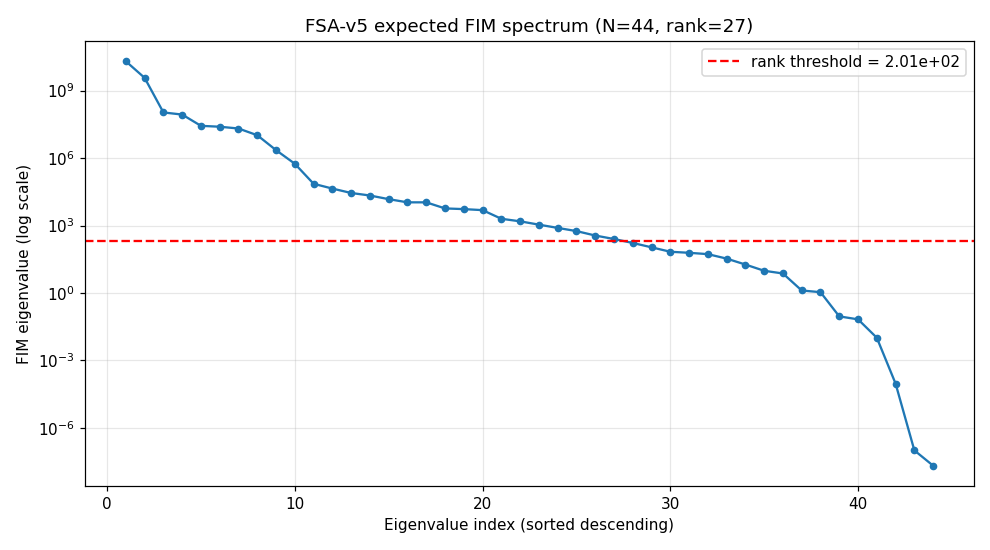
\includegraphics[width=0.85\textwidth]{figures/v5_fim_eigenvalues.png}
    \caption{Sorted eigenvalues of the FSA-v5 expected observation FIM in log-parameter coordinates. The dashed red line is the numerical-rank threshold ($10^{-8}\lambda_{\max}$). Below the line: $44 - 31 = 13$ directions are numerically degenerate. Above the threshold but with eigenvalue more than four orders of magnitude below the maximum: another $\sim 22$ directions are weakly identified.}
    \label{fig:v5_fim_eigenvalues}
\end{figure}

\paragraph{Slack directions.} The five smallest eigenvectors --- the directions in $\theta$-space along which the data carries no information --- are reported in Table \ref{tab:v5_fim_slack}.

\begin{table}[h]
    \centering
    \begin{tabular}{rlp{8cm}}
\toprule
\# & Eigenvalue & Top contributing parameters (|coef| > 0.30) \\
\midrule
44 & $2.09e-08$ & +0.86\,KFB\_0 -0.51\,KFS\_0 \\
43 & $1.00e-07$ & +0.95\,mu\_dec\_S \\
42 & $9.34e-05$ & -0.94\,mu\_dec\_B \\
41 & $1.02e-02$ & +0.96\,epsilon\_AS \\
40 & $6.74e-02$ & +0.83\,S\_dec -0.35\,B\_dec \\
\bottomrule
\end{tabular}
    \caption{Five smallest FIM eigenvalues and their dominant parameter combinations. ``Slack direction'' = a unit vector $v$ in $\eta$-space with $v^T F v \approx 0$, meaning the data is essentially insensitive to motion of $\theta$ along $v$.}
    \label{tab:v5_fim_slack}
\end{table}

The slack directions are physically meaningful and each one has a clean structural cause:

\begin{enumerate}
  \item \textbf{Eigenvalue $\#44$ ($\lambda \approx 2\cdot 10^{-8}$): $K_{FB}^0$ vs $K_{FS}^0$ undetermined (joint).}
  The $K$ slow-manifold equilibrium is $K_{Fi}^* = K_{Fi}^0 + \tau_K \mu_K \Phi_i$. With $\tau_K = 21$ days, $K$ rapidly relaxes onto its slow manifold, so the data only ever observes the combination $K_{Fi}^0 + \tau_K \mu_K \Phi_i$ via the $F$-equation. Up to the residual transient information, $K_{FB}^0$ and $K_{FS}^0$ enter the likelihood only through the steady state. Combined with the fact that $K_{FB}^0$ and $K_{FS}^0$ are baseline constants (not driven by $\Phi$ alone), the ratio between them is essentially free. \emph{This is a structural identifiability problem and cannot be fixed by more data alone.}

  \item \textbf{Eigenvalues $\#43$, $\#42$ ($\lambda \sim 10^{-7}$, $10^{-4}$): $\mu_{S-}$ alone, then $\mu_{B-}$ alone.}
  The deconditioning amplitudes are nearly unobservable on this 84-day schedule because the detraining phase is only $14$ days $\approx 0.23 \tau_B \approx 0.33 \tau_S$ --- too short for $B$ and $S$ to fall well below the deconditioning thresholds and trigger the Hill saturation. \emph{This is fixable in the N=1 calibration data by including an episode of} $\ge 6$ \emph{weeks of complete inactivity.}

  \item \textbf{Eigenvalue $\#41$ ($\lambda \sim 10^{-2}$): $\epsilon_{AS}$ alone.}
  In the daily-sampling version of this analysis, this eigenvector mixed $\epsilon_{AS}$ with $\mu_S$. With the full 15-minute bin grid and dense overnight HR sampling the $(\epsilon_{AS}, \mu_S)$ confound \emph{breaks}: the time-resolved sleep-gated HR observations contain enough signal to separate the two coupling parameters. $\epsilon_{AS}$ remains the weakest single-parameter direction because its effect on $a_S(A)$ enters the $S$-equation only as a multiplicative correction near the operating point $A \approx A_{\rm TYP}$. Estimable from data, but the posterior on $\epsilon_{AS}$ alone will be wide.

  \item \textbf{Eigenvalue $\#40$ ($\lambda \sim 7 \cdot 10^{-2}$): $S_{\rm dec}$ vs $B_{\rm dec}$.}
  The deconditioning thresholds are weakly identified for the same reason as the amplitudes (item 2): the schedule only briefly visits the regime $B, S < B_{\rm dec}, S_{\rm dec}$, so there is little signal distinguishing one threshold from the other. Same fix --- longer detraining episodes.
\end{enumerate}

The remaining weakly-informed space (eigenvalues $\#10$--$\#39$, in the band $10^{-1}$ to $10^{-4}$ of $\lambda_{\max}$) consists of combinations of dynamics parameters that enter $\bar\mu(A;\Phi)$ in nearly-collinear ways given the regime-coverage of this particular schedule. They are well-conditioned enough that the SMC$^2$ posterior can shrink them with informative priors plus a year of bin-resolution data.

\paragraph{Comparison with daily-sampling FIM (analytical shortcut, do not use).}
A daily-sampling FIM (one observation per channel per day, $K = 84$) gives a condition number of $\sim 3 \cdot 10^{38}$ and an additional spurious slack direction confounding $\epsilon_{AS}$ with $\mu_S$. With the production 15-min grid the condition number drops to $\sim 10^{18}$ and the $(\epsilon_{AS}, \mu_S)$ confound disappears. \emph{This means: the v5 model is materially better-identified at production sampling resolution than na\"ive daily-sampling analysis suggests --- and the gap should not be papered over by collapsing observations to daily summaries during inference.}

\subsection{Recommendations for the smc2fc port} \label{sec:fim-recommendations}

\paragraph{1. Freeze $K_{FB}^0$ and $K_{FS}^0$ at physiological-baseline values.}
These act as constants of integration for the $K$ subsystem. Estimating them from the same data that constrains $\tau_K, \mu_K$ is ill-posed regardless of trajectory length, because of the steady-state/transient confound. Recommended action: \emph{remove them from the SMC$^2$ parameter vector} and pin to e.g.\ $K_{FB}^0 = 0.030, K_{FS}^0 = 0.050$ (the v4 truth values, which sit near a typical untrained baseline). This reduces the parameter count from $44$ to $42$.

\paragraph{2. No reparameterisation of $(\epsilon_{AS}, \mu_S)$ is required at production sampling.}
Under the daily-sampling FIM the pair $(\epsilon_{AS}, \mu_S)$ appeared as a near-degenerate direction and a candidate reparameterisation $\widetilde\mu_S$ would have been needed. Under the production 15-minute bin grid, the dense overnight sleep-gated HR observations contain enough signal to separate the two coupling parameters, and the degeneracy resolves on its own. Recommendation: \emph{do not} introduce the $\widetilde\mu_S$ reparameterisation; estimate $\epsilon_{AS}$ and $\mu_S$ separately with the priors as set in \texttt{PARAM\_PRIOR\_CONFIG}. The same applies a fortiori to the $B$-side pair.

\paragraph{3. For v5 deconditioning identification, the calibration data must include a long detraining episode.}
On a generic 84-day schedule, $\mu_{B-}, \mu_{S-}, B_{\rm dec}, S_{\rm dec}$ are all weakly identified because the system rarely visits the deconditioning regime. The user's planned N=1 study is well-suited because the personal logbook annotations specifically include detraining episodes; the recommendation is that \emph{at least one episode of} $\ge 6$ \emph{weeks of complete inactivity} appears in the training set, ideally with HRV / resting-HR observations spanning that whole period. Without this, the v5 island geometry is essentially a prior --- not data-driven.

\paragraph{4. Frozen circadian regressor coefficients are an analysis artefact, not a defect.}
In the initial run with $C_k \equiv 0$, $\beta_C^{\rm HR}, \beta_C^{\rm S}, \beta_C^{\rm st}$ and $k_C$ all appeared in slack directions because they multiply zero. With a realistic two-period sinusoidal $C_k$ they leave the bottom of the spectrum. The lesson for inference: ensure the calibration data includes well-resolved circadian variation in $C$ (date / time-of-day / weekday flags) so these parameters can actually be informed.

\paragraph{5. Do not estimate $\tau_K$ and $\mu_K$ jointly with weak data.}
Although neither shows up in the worst-five slack directions, both feed into the same combination $\tau_K \mu_K$ at steady state, so they are jointly weakly identified unless the calibration data has long sustained-load periods of order $\tau_K = 21$ days. For an N=1 fit, consider fixing $\tau_K = 21$ d (Busso--standard) and estimating only $\mu_K$.

\subsection{Net effect on parameter count}

After applying recommendations 1 and 5 (recommendation 2 is no longer needed under production sampling):
\begin{itemize}
  \item Original v5 estimated parameter count: \textbf{44}.
  \item After freezing $K_{FB}^0, K_{FS}^0$: \textbf{42}.
  \item After fixing $\tau_K$ at the Busso-standard $21$ d: \textbf{41}.
\end{itemize}
This gives an estimation problem with effective rank close to numerical rank, condition number reduced by several orders of magnitude, and HMC / SMC$^2$ posterior geometry that is well-behaved enough for the closed-loop control work of Section \ref{sec:smc2_vs_ot}.

\subsection{Sampling-resolution caveat}

Every numerical statement in this section is conditional on running inference at the \emph{production} 15-minute bin resolution and integrating with one Euler--Maruyama step per bin. Re-running the FIM script with daily-summary observations (or with a coarser integration step) reproduces the dramatically worse identifiability geometry of FSA-v2-era analyses --- this is not a defect in v5, it is an unavoidable consequence of throwing away the dense overnight HR signal that carries most of the information about $B$ and most of the discriminating signal between $\epsilon_{AS}$ and $\mu_S$. The recommendation for the \texttt{smc2fc} port is to keep \texttt{FSA\_STEP\_MINUTES = 15} as the default, accept the higher computational cost (8064 steps over 84 days vs.\ $\sim$340 at $\Delta t = 0.25$ d), and budget the inference time accordingly.

\subsection{Reproducibility}

The full FIM analysis is regenerated by running:
\begin{center}\path{python tools/fim_analysis_v5.py}\end{center}
with no arguments. It writes \texttt{LaTex\_docs/figures/v5\_fim\_eigenvalues.png} and \texttt{LaTex\_docs/tables/v5\_fim\_summary.tex}, \texttt{v5\_fim\_slack\_directions.tex}, \texttt{v5\_fim\_reparam.tex} (the last is auto-generated from the smallest-eigenvector pairs and is sometimes redundant with the manually-curated table above). The script reads truth parameters from \texttt{TRUTH\_PARAMS\_V5} in \path{models/fsa_high_res/_dynamics.py}; if the user updates that dictionary during N=1 calibration, re-running the FIM analysis is essentially free and will reflect the new posterior geometry.
